\documentclass[twoside]{book}

% Packages required by doxygen
\usepackage{fixltx2e}
\usepackage{calc}
\usepackage{doxygen}
\usepackage[export]{adjustbox} % also loads graphicx
\usepackage{graphicx}
\usepackage[utf8]{inputenc}
\usepackage{makeidx}
\usepackage{multicol}
\usepackage{multirow}
\PassOptionsToPackage{warn}{textcomp}
\usepackage{textcomp}
\usepackage[nointegrals]{wasysym}
\usepackage[table]{xcolor}

% Font selection
\usepackage[T1]{fontenc}
\usepackage[scaled=.90]{helvet}
\usepackage{courier}
\usepackage{amssymb}
\usepackage{sectsty}
\renewcommand{\familydefault}{\sfdefault}
\allsectionsfont{%
  \fontseries{bc}\selectfont%
  \color{darkgray}%
}
\renewcommand{\DoxyLabelFont}{%
  \fontseries{bc}\selectfont%
  \color{darkgray}%
}
\newcommand{\+}{\discretionary{\mbox{\scriptsize$\hookleftarrow$}}{}{}}

% Page & text layout
\usepackage{geometry}
\geometry{%
  a4paper,%
  top=2.5cm,%
  bottom=2.5cm,%
  left=2.5cm,%
  right=2.5cm%
}
\tolerance=750
\hfuzz=15pt
\hbadness=750
\setlength{\emergencystretch}{15pt}
\setlength{\parindent}{0cm}
\setlength{\parskip}{3ex plus 2ex minus 2ex}
\makeatletter
\renewcommand{\paragraph}{%
  \@startsection{paragraph}{4}{0ex}{-1.0ex}{1.0ex}{%
    \normalfont\normalsize\bfseries\SS@parafont%
  }%
}
\renewcommand{\subparagraph}{%
  \@startsection{subparagraph}{5}{0ex}{-1.0ex}{1.0ex}{%
    \normalfont\normalsize\bfseries\SS@subparafont%
  }%
}
\makeatother

% Headers & footers
\usepackage{fancyhdr}
\pagestyle{fancyplain}
\fancyhead[LE]{\fancyplain{}{\bfseries\thepage}}
\fancyhead[CE]{\fancyplain{}{}}
\fancyhead[RE]{\fancyplain{}{\bfseries\leftmark}}
\fancyhead[LO]{\fancyplain{}{\bfseries\rightmark}}
\fancyhead[CO]{\fancyplain{}{}}
\fancyhead[RO]{\fancyplain{}{\bfseries\thepage}}
\fancyfoot[LE]{\fancyplain{}{}}
\fancyfoot[CE]{\fancyplain{}{}}
\fancyfoot[RE]{\fancyplain{}{\bfseries\scriptsize Generated by Doxygen }}
\fancyfoot[LO]{\fancyplain{}{\bfseries\scriptsize Generated by Doxygen }}
\fancyfoot[CO]{\fancyplain{}{}}
\fancyfoot[RO]{\fancyplain{}{}}
\renewcommand{\footrulewidth}{0.4pt}
\renewcommand{\chaptermark}[1]{%
  \markboth{#1}{}%
}
\renewcommand{\sectionmark}[1]{%
  \markright{\thesection\ #1}%
}

% Indices & bibliography
\usepackage{natbib}
\usepackage[titles]{tocloft}
\setcounter{tocdepth}{3}
\setcounter{secnumdepth}{5}
\makeindex

% Hyperlinks (required, but should be loaded last)
\usepackage{ifpdf}
\ifpdf
  \usepackage[pdftex,pagebackref=true]{hyperref}
\else
  \usepackage[ps2pdf,pagebackref=true]{hyperref}
\fi
\hypersetup{%
  colorlinks=true,%
  linkcolor=blue,%
  citecolor=blue,%
  unicode%
}

% Custom commands
\newcommand{\clearemptydoublepage}{%
  \newpage{\pagestyle{empty}\cleardoublepage}%
}

\usepackage{caption}
\captionsetup{labelsep=space,justification=centering,font={bf},singlelinecheck=off,skip=4pt,position=top}

%===== C O N T E N T S =====

\begin{document}

% Titlepage & ToC
\hypersetup{pageanchor=false,
             bookmarksnumbered=true,
             pdfencoding=unicode
            }
\pagenumbering{alph}
\begin{titlepage}
\vspace*{7cm}
\begin{center}%
{\Large Hangman }\\
\vspace*{1cm}
{\large Generated by Doxygen 1.8.13}\\
\end{center}
\end{titlepage}
\clearemptydoublepage
\pagenumbering{roman}
\tableofcontents
\clearemptydoublepage
\pagenumbering{arabic}
\hypersetup{pageanchor=true}

%--- Begin generated contents ---
\chapter{Project H\+A\+N\+G\+M\+AN -\/ Official documentation}
\label{index}\hypertarget{index}{}\begin{DoxyAuthor}{Author}
Patrick Rotter 
\end{DoxyAuthor}
\begin{DoxyVersion}{Version}
1.\+0 
\end{DoxyVersion}
\begin{DoxyDate}{Date}
16.\+01.\+2021
\end{DoxyDate}
\hypertarget{index_description}{}\section{Project description}\label{index_description}
This project represents the classic game \char`\"{}\+Hangman\char`\"{}. The player is provided a secret word and tries to guess it by suggesting letters within a certain number of guesses. 
\chapter{File Index}
\section{File List}
Here is a list of all files with brief descriptions\+:\begin{DoxyCompactList}
\item\contentsline{section}{/home/osboxes/eclipse-\/workspace/125\+\_\+hangman/\hyperlink{hangman__functions_8c}{hangman\+\_\+functions.\+c} }{\pageref{hangman__functions_8c}}{}
\item\contentsline{section}{/home/osboxes/eclipse-\/workspace/125\+\_\+hangman/\hyperlink{hangman__header_8h}{hangman\+\_\+header.\+h} }{\pageref{hangman__header_8h}}{}
\item\contentsline{section}{/home/osboxes/eclipse-\/workspace/125\+\_\+hangman/\hyperlink{hangman__main_8c}{hangman\+\_\+main.\+c} }{\pageref{hangman__main_8c}}{}
\end{DoxyCompactList}

\chapter{File Documentation}
\hypertarget{hangman__functions_8c}{}\section{/home/osboxes/eclipse-\/workspace/125\+\_\+hangman/hangman\+\_\+functions.c File Reference}
\label{hangman__functions_8c}\index{/home/osboxes/eclipse-\/workspace/125\+\_\+hangman/hangman\+\_\+functions.\+c@{/home/osboxes/eclipse-\/workspace/125\+\_\+hangman/hangman\+\_\+functions.\+c}}
{\ttfamily \#include \char`\"{}hangman\+\_\+header.\+h\char`\"{}}\newline
Include dependency graph for hangman\+\_\+functions.\+c\+:
\nopagebreak
\begin{figure}[H]
\begin{center}
\leavevmode
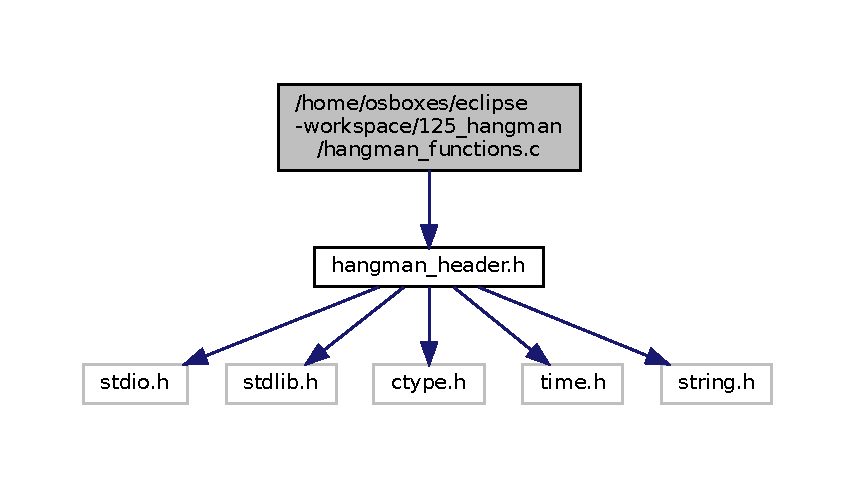
\includegraphics[width=350pt]{hangman__functions_8c__incl}
\end{center}
\end{figure}
\subsection*{Functions}
\begin{DoxyCompactItemize}
\item 
int \hyperlink{hangman__functions_8c_a9677dd5ca6faade6e5c0704065cb97bb}{word\+Already\+Used} (int total\+Words, char $\ast$word\+To\+Guess)
\begin{DoxyCompactList}\small\item\em Checks, if a selected word has been chosen already and resets the process. \end{DoxyCompactList}\item 
void \hyperlink{hangman__functions_8c_a5e7c8c35c652cf16af647f8cfebbcac8}{print\+Guessing\+Bank} (char $\ast$guessing\+Bank)
\begin{DoxyCompactList}\small\item\em Prints incorrectly guessed letters (\char`\"{}guessing bank\char`\"{}) to stdout. \end{DoxyCompactList}\item 
void \hyperlink{hangman__functions_8c_abc2b9ff2282166cb3ef1ccdf09381c57}{check\+File} (F\+I\+LE $\ast$p\+File)
\begin{DoxyCompactList}\small\item\em Checks, if a provided file was opened successfully. \end{DoxyCompactList}\item 
void \hyperlink{hangman__functions_8c_a484be6c6a44525057d3caf6537d99389}{print\+Board} (int position, F\+I\+LE $\ast$p\+Log, char $\ast$board, char $\ast$blanks, char $\ast$guessing\+Bank)
\begin{DoxyCompactList}\small\item\em Prints the stick figure and the game board. \end{DoxyCompactList}\item 
char \hyperlink{hangman__functions_8c_a5f67ce8a708479e4b2a709c62c85bd57}{read\+User\+Guess} (F\+I\+LE $\ast$p\+Log, char $\ast$word\+To\+Guess)
\begin{DoxyCompactList}\small\item\em Scans and checks user guess and returns it to main. \end{DoxyCompactList}\item 
int \hyperlink{hangman__functions_8c_a002731390fffa21fb1cd9163780b5bbd}{is\+Already\+Guessed} (int position, char guess, char $\ast$guessing\+Bank)
\begin{DoxyCompactList}\small\item\em Checks with subfunction \hyperlink{hangman__header_8h_af2811c2f6f7b18dafc51839dd18bd93a}{is\+In\+Word()}, if entered letter is part of the guessing bank of incorrect letters. \end{DoxyCompactList}\item 
int \hyperlink{hangman__functions_8c_aec373c0279bea07cf6d6c95833c2396c}{check\+User\+Guess} (int word\+Length, char guess, char $\ast$word\+To\+Guess, char $\ast$blanks)
\begin{DoxyCompactList}\small\item\em Checks, if entered letter is in secret word and replaces blank with correctly entered letter. \end{DoxyCompactList}\item 
int \hyperlink{hangman__functions_8c_aa25d103659434a0526d7cc1c12aea543}{play\+Again} ()
\begin{DoxyCompactList}\small\item\em Asks the user, if they want to play again. \end{DoxyCompactList}\item 
int \hyperlink{hangman__functions_8c_ad517f8e00c44f43c59b252b47fc8822c}{check\+If\+Won} (F\+I\+LE $\ast$p\+Log, char $\ast$word\+To\+Guess, char $\ast$blanks)
\begin{DoxyCompactList}\small\item\em Checks, if the player has won the game. \end{DoxyCompactList}\item 
int \hyperlink{hangman__functions_8c_af2811c2f6f7b18dafc51839dd18bd93a}{is\+In\+Word} (int position, char guess, char $\ast$guessing\+Bank)
\begin{DoxyCompactList}\small\item\em Checks, if entered letter is part of the guessing bank of incorrect letters. Subfunction of \hyperlink{hangman__header_8h_a002731390fffa21fb1cd9163780b5bbd}{is\+Already\+Guessed()} \end{DoxyCompactList}\item 
void \hyperlink{hangman__functions_8c_ad109742c0784a0379d5911bce804a088}{pick\+Word} (int $\ast$word\+Length, F\+I\+LE $\ast$p\+Word\+File, int total\+Words, char $\ast$$\ast$word\+To\+Guess, char $\ast$$\ast$blanks, char $\ast$$\ast$guessing\+Bank)
\begin{DoxyCompactList}\small\item\em Picks a random word from a provided list of words. \end{DoxyCompactList}\end{DoxyCompactItemize}


\subsection{Function Documentation}
\mbox{\Hypertarget{hangman__functions_8c_abc2b9ff2282166cb3ef1ccdf09381c57}\label{hangman__functions_8c_abc2b9ff2282166cb3ef1ccdf09381c57}} 
\index{hangman\+\_\+functions.\+c@{hangman\+\_\+functions.\+c}!check\+File@{check\+File}}
\index{check\+File@{check\+File}!hangman\+\_\+functions.\+c@{hangman\+\_\+functions.\+c}}
\subsubsection{\texorpdfstring{check\+File()}{checkFile()}}
{\footnotesize\ttfamily void check\+File (\begin{DoxyParamCaption}\item[{F\+I\+LE $\ast$}]{p\+File }\end{DoxyParamCaption})}



Checks, if a provided file was opened successfully. 


\begin{DoxyParams}{Parameters}
{\em $\ast$p\+File} & Word input file\\
\hline
\end{DoxyParams}
If file pointer is N\+U\+LL, program exits with unsuccessful termination. \mbox{\Hypertarget{hangman__functions_8c_ad517f8e00c44f43c59b252b47fc8822c}\label{hangman__functions_8c_ad517f8e00c44f43c59b252b47fc8822c}} 
\index{hangman\+\_\+functions.\+c@{hangman\+\_\+functions.\+c}!check\+If\+Won@{check\+If\+Won}}
\index{check\+If\+Won@{check\+If\+Won}!hangman\+\_\+functions.\+c@{hangman\+\_\+functions.\+c}}
\subsubsection{\texorpdfstring{check\+If\+Won()}{checkIfWon()}}
{\footnotesize\ttfamily int check\+If\+Won (\begin{DoxyParamCaption}\item[{F\+I\+LE $\ast$}]{p\+Log,  }\item[{char $\ast$}]{word\+To\+Guess,  }\item[{char $\ast$}]{blanks }\end{DoxyParamCaption})}



Checks, if the player has won the game. 


\begin{DoxyParams}{Parameters}
{\em $\ast$p\+Log} & Log file \\
\hline
{\em $\ast$word\+To\+Guess} & Secret Hangman word \\
\hline
{\em $\ast$blanks} & Saves blanks and correctly guessed letters\\
\hline
\end{DoxyParams}
If the secret word and all entered letters (that represent the secret word) match, the user wins. Prints a winning message to stdout and the current time and secret word into the log file. \begin{DoxyReturn}{Returns}
1 If user won the game 

0 If user has not yet won the game 
\end{DoxyReturn}
\mbox{\Hypertarget{hangman__functions_8c_aec373c0279bea07cf6d6c95833c2396c}\label{hangman__functions_8c_aec373c0279bea07cf6d6c95833c2396c}} 
\index{hangman\+\_\+functions.\+c@{hangman\+\_\+functions.\+c}!check\+User\+Guess@{check\+User\+Guess}}
\index{check\+User\+Guess@{check\+User\+Guess}!hangman\+\_\+functions.\+c@{hangman\+\_\+functions.\+c}}
\subsubsection{\texorpdfstring{check\+User\+Guess()}{checkUserGuess()}}
{\footnotesize\ttfamily int check\+User\+Guess (\begin{DoxyParamCaption}\item[{int}]{word\+Length,  }\item[{char}]{guess,  }\item[{char $\ast$}]{word\+To\+Guess,  }\item[{char $\ast$}]{blanks }\end{DoxyParamCaption})}



Checks, if entered letter is in secret word and replaces blank with correctly entered letter. 


\begin{DoxyParams}{Parameters}
{\em word\+Length} & Length of secret word \\
\hline
{\em guess} & User guess \\
\hline
{\em $\ast$word\+To\+Guess} & Secret Hangman word \\
\hline
{\em $\ast$blanks} & Saves blanks and correctly guessed letters \\
\hline
\end{DoxyParams}
\begin{DoxyReturn}{Returns}
1 If entered letter is in secret word 

0 If entered letter is not in secret word 
\end{DoxyReturn}
\mbox{\Hypertarget{hangman__functions_8c_a002731390fffa21fb1cd9163780b5bbd}\label{hangman__functions_8c_a002731390fffa21fb1cd9163780b5bbd}} 
\index{hangman\+\_\+functions.\+c@{hangman\+\_\+functions.\+c}!is\+Already\+Guessed@{is\+Already\+Guessed}}
\index{is\+Already\+Guessed@{is\+Already\+Guessed}!hangman\+\_\+functions.\+c@{hangman\+\_\+functions.\+c}}
\subsubsection{\texorpdfstring{is\+Already\+Guessed()}{isAlreadyGuessed()}}
{\footnotesize\ttfamily int is\+Already\+Guessed (\begin{DoxyParamCaption}\item[{int}]{position,  }\item[{char}]{guess,  }\item[{char $\ast$}]{guessing\+Bank }\end{DoxyParamCaption})}



Checks with subfunction \hyperlink{hangman__header_8h_af2811c2f6f7b18dafc51839dd18bd93a}{is\+In\+Word()}, if entered letter is part of the guessing bank of incorrect letters. 


\begin{DoxyParams}{Parameters}
{\em position} & Counter for incorrectly entered letters \\
\hline
{\em guess} & User guess \\
\hline
{\em $\ast$guessing\+Bank} & Saves incorrectly guessed letters \\
\hline
\end{DoxyParams}
\begin{DoxyReturn}{Returns}
1 If entered letter is in guessing bank/already guessed 

0 If entered letter is not in guessing bank/already guessed 
\end{DoxyReturn}
\mbox{\Hypertarget{hangman__functions_8c_af2811c2f6f7b18dafc51839dd18bd93a}\label{hangman__functions_8c_af2811c2f6f7b18dafc51839dd18bd93a}} 
\index{hangman\+\_\+functions.\+c@{hangman\+\_\+functions.\+c}!is\+In\+Word@{is\+In\+Word}}
\index{is\+In\+Word@{is\+In\+Word}!hangman\+\_\+functions.\+c@{hangman\+\_\+functions.\+c}}
\subsubsection{\texorpdfstring{is\+In\+Word()}{isInWord()}}
{\footnotesize\ttfamily int is\+In\+Word (\begin{DoxyParamCaption}\item[{int}]{position,  }\item[{char}]{guess,  }\item[{char $\ast$}]{guessing\+Bank }\end{DoxyParamCaption})}



Checks, if entered letter is part of the guessing bank of incorrect letters. Subfunction of \hyperlink{hangman__header_8h_a002731390fffa21fb1cd9163780b5bbd}{is\+Already\+Guessed()} 


\begin{DoxyParams}{Parameters}
{\em position} & Counter for incorrectly entered letters \\
\hline
{\em guess} & User guess \\
\hline
{\em $\ast$guessing\+Bank} & Saves incorrectly guessed letters \\
\hline
\end{DoxyParams}
\begin{DoxyReturn}{Returns}
1 If entered letter is in guessing bank/already guessed 

0 If entered letter is not in guessing bank/already guessed 
\end{DoxyReturn}
\mbox{\Hypertarget{hangman__functions_8c_ad109742c0784a0379d5911bce804a088}\label{hangman__functions_8c_ad109742c0784a0379d5911bce804a088}} 
\index{hangman\+\_\+functions.\+c@{hangman\+\_\+functions.\+c}!pick\+Word@{pick\+Word}}
\index{pick\+Word@{pick\+Word}!hangman\+\_\+functions.\+c@{hangman\+\_\+functions.\+c}}
\subsubsection{\texorpdfstring{pick\+Word()}{pickWord()}}
{\footnotesize\ttfamily void pick\+Word (\begin{DoxyParamCaption}\item[{int $\ast$}]{word\+Length,  }\item[{F\+I\+LE $\ast$}]{p\+Word\+File,  }\item[{int}]{total\+Words,  }\item[{char $\ast$$\ast$}]{word\+To\+Guess,  }\item[{char $\ast$$\ast$}]{blanks,  }\item[{char $\ast$$\ast$}]{guessing\+Bank }\end{DoxyParamCaption})}



Picks a random word from a provided list of words. 


\begin{DoxyParams}{Parameters}
{\em $\ast$word\+Length} & Length of the chosen word \\
\hline
{\em $\ast$p\+Word\+File} & File with list of words \\
\hline
{\em $\ast$total\+Words} & Total words read in from file \\
\hline
{\em $\ast$$\ast$word\+To\+Guess} & Secret Hangman word \\
\hline
{\em $\ast$$\ast$blanks} & Saves blanks and correctly guessed letters \\
\hline
{\em $\ast$$\ast$guessing\+Bank} & Saves incorrectly guessed letters\\
\hline
\end{DoxyParams}
Randomly chooses a word by selecting a random number between 1 and total\+Words. Reads the amount of characters of chosen secret word in and allocates memory for the secret word, blanks and the guessing bank. Scans the word from the file and capitalizes it. Lastly initializes blanks and guessing bank arrays. \mbox{\Hypertarget{hangman__functions_8c_aa25d103659434a0526d7cc1c12aea543}\label{hangman__functions_8c_aa25d103659434a0526d7cc1c12aea543}} 
\index{hangman\+\_\+functions.\+c@{hangman\+\_\+functions.\+c}!play\+Again@{play\+Again}}
\index{play\+Again@{play\+Again}!hangman\+\_\+functions.\+c@{hangman\+\_\+functions.\+c}}
\subsubsection{\texorpdfstring{play\+Again()}{playAgain()}}
{\footnotesize\ttfamily int play\+Again (\begin{DoxyParamCaption}{ }\end{DoxyParamCaption})}



Asks the user, if they want to play again. 

Reads in user input after the question if they want to play again.

3 options\+:
\begin{DoxyEnumerate}
\item Y to play again -\/ Resets game and restarts game loop.
\item N to quit -\/ Exits the game.
\item Invalid input -\/ Message appears to enter valid input. \begin{DoxyReturn}{Returns}
1 if Y 

0 if N 

\hyperlink{hangman__header_8h_aa25d103659434a0526d7cc1c12aea543}{play\+Again()} if user entered invalid input 
\end{DoxyReturn}

\end{DoxyEnumerate}\mbox{\Hypertarget{hangman__functions_8c_a484be6c6a44525057d3caf6537d99389}\label{hangman__functions_8c_a484be6c6a44525057d3caf6537d99389}} 
\index{hangman\+\_\+functions.\+c@{hangman\+\_\+functions.\+c}!print\+Board@{print\+Board}}
\index{print\+Board@{print\+Board}!hangman\+\_\+functions.\+c@{hangman\+\_\+functions.\+c}}
\subsubsection{\texorpdfstring{print\+Board()}{printBoard()}}
{\footnotesize\ttfamily void print\+Board (\begin{DoxyParamCaption}\item[{int}]{position,  }\item[{F\+I\+LE $\ast$}]{p\+Log,  }\item[{char $\ast$}]{board,  }\item[{char $\ast$}]{blanks,  }\item[{char $\ast$}]{guessing\+Bank }\end{DoxyParamCaption})}



Prints the stick figure and the game board. 


\begin{DoxyParams}{Parameters}
{\em position} & Counter for incorrectly entered letters \\
\hline
{\em $\ast$p\+Log} & Log file \\
\hline
{\em $\ast$board} & Hangman stick figure \\
\hline
{\em $\ast$blanks} & Saves blanks and correctly guessed letters \\
\hline
{\em $\ast$guessing\+Bank} & Saves incorrectly guessed letters\\
\hline
\end{DoxyParams}
Prints stick figure to stdout and game board to stdout and log file. Calls function \hyperlink{hangman__header_8h_a5e7c8c35c652cf16af647f8cfebbcac8}{print\+Guessing\+Bank()} to print incorrect letters to stdout \mbox{\Hypertarget{hangman__functions_8c_a5e7c8c35c652cf16af647f8cfebbcac8}\label{hangman__functions_8c_a5e7c8c35c652cf16af647f8cfebbcac8}} 
\index{hangman\+\_\+functions.\+c@{hangman\+\_\+functions.\+c}!print\+Guessing\+Bank@{print\+Guessing\+Bank}}
\index{print\+Guessing\+Bank@{print\+Guessing\+Bank}!hangman\+\_\+functions.\+c@{hangman\+\_\+functions.\+c}}
\subsubsection{\texorpdfstring{print\+Guessing\+Bank()}{printGuessingBank()}}
{\footnotesize\ttfamily void print\+Guessing\+Bank (\begin{DoxyParamCaption}\item[{char $\ast$}]{guessing\+Bank }\end{DoxyParamCaption})}



Prints incorrectly guessed letters (\char`\"{}guessing bank\char`\"{}) to stdout. 


\begin{DoxyParams}{Parameters}
{\em $\ast$guessing\+Bank} & Saves incorrectly guessed letters \\
\hline
\end{DoxyParams}
\mbox{\Hypertarget{hangman__functions_8c_a5f67ce8a708479e4b2a709c62c85bd57}\label{hangman__functions_8c_a5f67ce8a708479e4b2a709c62c85bd57}} 
\index{hangman\+\_\+functions.\+c@{hangman\+\_\+functions.\+c}!read\+User\+Guess@{read\+User\+Guess}}
\index{read\+User\+Guess@{read\+User\+Guess}!hangman\+\_\+functions.\+c@{hangman\+\_\+functions.\+c}}
\subsubsection{\texorpdfstring{read\+User\+Guess()}{readUserGuess()}}
{\footnotesize\ttfamily char read\+User\+Guess (\begin{DoxyParamCaption}\item[{F\+I\+LE $\ast$}]{p\+Log,  }\item[{char $\ast$}]{word\+To\+Guess }\end{DoxyParamCaption})}



Scans and checks user guess and returns it to main. 


\begin{DoxyParams}{Parameters}
{\em $\ast$p\+Log} & Log file \\
\hline
{\em $\ast$word\+To\+Guess} & Secret Hangman word\\
\hline
\end{DoxyParams}
Asks the user to enter a letter and capitalizes input. Writes current time into log file.

4 options\+:
\begin{DoxyEnumerate}
\item If user manages to guess the whole word, they instantly win the round and the game restarts.
\item If user inputs more than 1 character and fail to guess the secret word it\textquotesingle{}s \char`\"{}\+Game over\char`\"{}.
\item If user input is 1 alphabetic character, the entered character is returned.
\item If user input is 1 non-\/alphabetic character a message appears and the function restarts. \begin{DoxyReturn}{Returns}
guess\mbox{[}0\mbox{]} = 0 with option 1. and 2. -\/ game restarts in \hyperlink{hangman__main_8c_a0ddf1224851353fc92bfbff6f499fa97}{main()} 

guess\mbox{[}0\mbox{]} if user enters an alphabetic character 

\hyperlink{hangman__header_8h_aec373c0279bea07cf6d6c95833c2396c}{check\+User\+Guess()} if user enters non-\/alphabetic character 
\end{DoxyReturn}

\end{DoxyEnumerate}\mbox{\Hypertarget{hangman__functions_8c_a9677dd5ca6faade6e5c0704065cb97bb}\label{hangman__functions_8c_a9677dd5ca6faade6e5c0704065cb97bb}} 
\index{hangman\+\_\+functions.\+c@{hangman\+\_\+functions.\+c}!word\+Already\+Used@{word\+Already\+Used}}
\index{word\+Already\+Used@{word\+Already\+Used}!hangman\+\_\+functions.\+c@{hangman\+\_\+functions.\+c}}
\subsubsection{\texorpdfstring{word\+Already\+Used()}{wordAlreadyUsed()}}
{\footnotesize\ttfamily int word\+Already\+Used (\begin{DoxyParamCaption}\item[{int}]{total\+Words,  }\item[{char $\ast$}]{word\+To\+Guess }\end{DoxyParamCaption})}



Checks, if a selected word has been chosen already and resets the process. 


\begin{DoxyParams}{Parameters}
{\em $\ast$word\+To\+Guess} & Secret Hangman word \\
\hline
\end{DoxyParams}
\begin{DoxyReturn}{Returns}
1 If a word has been selected already 

0 If a word has not yet been selected 
\end{DoxyReturn}

\hypertarget{hangman__header_8h}{}\section{/home/osboxes/eclipse-\/workspace/125\+\_\+hangman/hangman\+\_\+header.h File Reference}
\label{hangman__header_8h}\index{/home/osboxes/eclipse-\/workspace/125\+\_\+hangman/hangman\+\_\+header.\+h@{/home/osboxes/eclipse-\/workspace/125\+\_\+hangman/hangman\+\_\+header.\+h}}
{\ttfamily \#include $<$stdio.\+h$>$}\newline
{\ttfamily \#include $<$stdlib.\+h$>$}\newline
{\ttfamily \#include $<$ctype.\+h$>$}\newline
{\ttfamily \#include $<$time.\+h$>$}\newline
{\ttfamily \#include $<$string.\+h$>$}\newline
Include dependency graph for hangman\+\_\+header.\+h\+:
\nopagebreak
\begin{figure}[H]
\begin{center}
\leavevmode
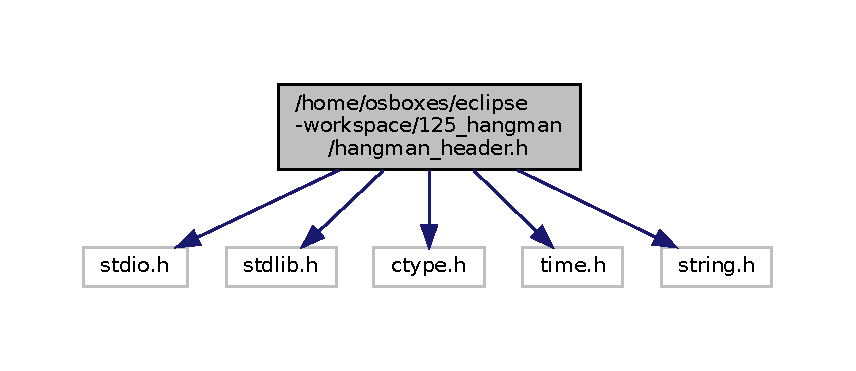
\includegraphics[width=350pt]{hangman__header_8h__incl}
\end{center}
\end{figure}
This graph shows which files directly or indirectly include this file\+:
\nopagebreak
\begin{figure}[H]
\begin{center}
\leavevmode
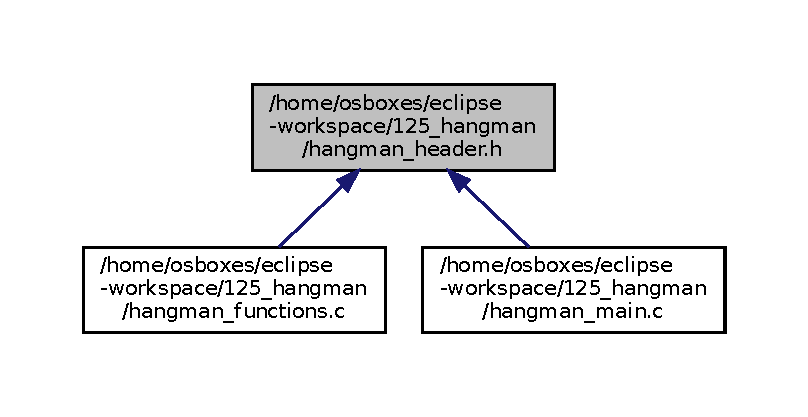
\includegraphics[width=350pt]{hangman__header_8h__dep__incl}
\end{center}
\end{figure}
\subsection*{Macros}
\begin{DoxyCompactItemize}
\item 
\#define \hyperlink{hangman__header_8h_ac8c4d8667136ad6b8c5936106a240ec7}{L\+I\+V\+ES}~7
\item 
\#define \hyperlink{hangman__header_8h_a7e7e22324965cdba939a9dc4afdb9189}{M\+A\+X\+C\+H\+A\+R\+A\+C\+T\+E\+RS}~64
\item 
\#define \hyperlink{hangman__header_8h_ae888bad586ab55d3ddc7c96ad1430734}{M\+A\+X\+F\+I\+L\+E\+N\+A\+M\+E\+L\+E\+N\+G\+TH}~101
\item 
\#define \hyperlink{hangman__header_8h_af9b7df044879d287753130096834a4f7}{M\+A\+X\+S\+A\+V\+E\+D\+W\+O\+R\+DS}~100
\end{DoxyCompactItemize}
\subsection*{Functions}
\begin{DoxyCompactItemize}
\item 
void \hyperlink{hangman__header_8h_abc2b9ff2282166cb3ef1ccdf09381c57}{check\+File} (F\+I\+LE $\ast$p\+File)
\begin{DoxyCompactList}\small\item\em Checks, if a provided file was opened successfully. \end{DoxyCompactList}\item 
char \hyperlink{hangman__header_8h_a5f67ce8a708479e4b2a709c62c85bd57}{read\+User\+Guess} (F\+I\+LE $\ast$p\+Log, char $\ast$word\+To\+Guess)
\begin{DoxyCompactList}\small\item\em Scans and checks user guess and returns it to main. \end{DoxyCompactList}\item 
int \hyperlink{hangman__header_8h_a002731390fffa21fb1cd9163780b5bbd}{is\+Already\+Guessed} (int position, char guess, char $\ast$guessing\+Bank)
\begin{DoxyCompactList}\small\item\em Checks with subfunction \hyperlink{hangman__header_8h_af2811c2f6f7b18dafc51839dd18bd93a}{is\+In\+Word()}, if entered letter is part of the guessing bank of incorrect letters. \end{DoxyCompactList}\item 
int \hyperlink{hangman__header_8h_aec373c0279bea07cf6d6c95833c2396c}{check\+User\+Guess} (int word\+Length, char guess, char $\ast$word\+To\+Guess, char $\ast$blanks)
\begin{DoxyCompactList}\small\item\em Checks, if entered letter is in secret word and replaces blank with correctly entered letter. \end{DoxyCompactList}\item 
int \hyperlink{hangman__header_8h_ad517f8e00c44f43c59b252b47fc8822c}{check\+If\+Won} (F\+I\+LE $\ast$p\+Log, char $\ast$word\+To\+Guess, char $\ast$blanks)
\begin{DoxyCompactList}\small\item\em Checks, if the player has won the game. \end{DoxyCompactList}\item 
void \hyperlink{hangman__header_8h_a484be6c6a44525057d3caf6537d99389}{print\+Board} (int position, F\+I\+LE $\ast$p\+Log, char $\ast$board, char $\ast$blanks, char $\ast$guessing\+Bank)
\begin{DoxyCompactList}\small\item\em Prints the stick figure and the game board. \end{DoxyCompactList}\item 
void \hyperlink{hangman__header_8h_ad109742c0784a0379d5911bce804a088}{pick\+Word} (int $\ast$word\+Length, F\+I\+LE $\ast$p\+Word\+File, int total\+Words, char $\ast$$\ast$word\+To\+Guess, char $\ast$$\ast$blanks, char $\ast$$\ast$guessing\+Bank)
\begin{DoxyCompactList}\small\item\em Picks a random word from a provided list of words. \end{DoxyCompactList}\item 
int \hyperlink{hangman__header_8h_aa25d103659434a0526d7cc1c12aea543}{play\+Again} ()
\begin{DoxyCompactList}\small\item\em Asks the user, if they want to play again. \end{DoxyCompactList}\item 
int \hyperlink{hangman__header_8h_af2811c2f6f7b18dafc51839dd18bd93a}{is\+In\+Word} (int position, char guess, char $\ast$guessing\+Bank)
\begin{DoxyCompactList}\small\item\em Checks, if entered letter is part of the guessing bank of incorrect letters. Subfunction of \hyperlink{hangman__header_8h_a002731390fffa21fb1cd9163780b5bbd}{is\+Already\+Guessed()} \end{DoxyCompactList}\item 
void \hyperlink{hangman__header_8h_a5e7c8c35c652cf16af647f8cfebbcac8}{print\+Guessing\+Bank} (char $\ast$guessing\+Bank)
\begin{DoxyCompactList}\small\item\em Prints incorrectly guessed letters (\char`\"{}guessing bank\char`\"{}) to stdout. \end{DoxyCompactList}\item 
int \hyperlink{hangman__header_8h_a9677dd5ca6faade6e5c0704065cb97bb}{word\+Already\+Used} (int total\+Words, char $\ast$word\+To\+Guess)
\begin{DoxyCompactList}\small\item\em Checks, if a selected word has been chosen already and resets the process. \end{DoxyCompactList}\end{DoxyCompactItemize}


\subsection{Macro Definition Documentation}
\mbox{\Hypertarget{hangman__header_8h_ac8c4d8667136ad6b8c5936106a240ec7}\label{hangman__header_8h_ac8c4d8667136ad6b8c5936106a240ec7}} 
\index{hangman\+\_\+header.\+h@{hangman\+\_\+header.\+h}!L\+I\+V\+ES@{L\+I\+V\+ES}}
\index{L\+I\+V\+ES@{L\+I\+V\+ES}!hangman\+\_\+header.\+h@{hangman\+\_\+header.\+h}}
\subsubsection{\texorpdfstring{L\+I\+V\+ES}{LIVES}}
{\footnotesize\ttfamily \#define L\+I\+V\+ES~7}

\mbox{\Hypertarget{hangman__header_8h_a7e7e22324965cdba939a9dc4afdb9189}\label{hangman__header_8h_a7e7e22324965cdba939a9dc4afdb9189}} 
\index{hangman\+\_\+header.\+h@{hangman\+\_\+header.\+h}!M\+A\+X\+C\+H\+A\+R\+A\+C\+T\+E\+RS@{M\+A\+X\+C\+H\+A\+R\+A\+C\+T\+E\+RS}}
\index{M\+A\+X\+C\+H\+A\+R\+A\+C\+T\+E\+RS@{M\+A\+X\+C\+H\+A\+R\+A\+C\+T\+E\+RS}!hangman\+\_\+header.\+h@{hangman\+\_\+header.\+h}}
\subsubsection{\texorpdfstring{M\+A\+X\+C\+H\+A\+R\+A\+C\+T\+E\+RS}{MAXCHARACTERS}}
{\footnotesize\ttfamily \#define M\+A\+X\+C\+H\+A\+R\+A\+C\+T\+E\+RS~64}

\mbox{\Hypertarget{hangman__header_8h_ae888bad586ab55d3ddc7c96ad1430734}\label{hangman__header_8h_ae888bad586ab55d3ddc7c96ad1430734}} 
\index{hangman\+\_\+header.\+h@{hangman\+\_\+header.\+h}!M\+A\+X\+F\+I\+L\+E\+N\+A\+M\+E\+L\+E\+N\+G\+TH@{M\+A\+X\+F\+I\+L\+E\+N\+A\+M\+E\+L\+E\+N\+G\+TH}}
\index{M\+A\+X\+F\+I\+L\+E\+N\+A\+M\+E\+L\+E\+N\+G\+TH@{M\+A\+X\+F\+I\+L\+E\+N\+A\+M\+E\+L\+E\+N\+G\+TH}!hangman\+\_\+header.\+h@{hangman\+\_\+header.\+h}}
\subsubsection{\texorpdfstring{M\+A\+X\+F\+I\+L\+E\+N\+A\+M\+E\+L\+E\+N\+G\+TH}{MAXFILENAMELENGTH}}
{\footnotesize\ttfamily \#define M\+A\+X\+F\+I\+L\+E\+N\+A\+M\+E\+L\+E\+N\+G\+TH~101}

\mbox{\Hypertarget{hangman__header_8h_af9b7df044879d287753130096834a4f7}\label{hangman__header_8h_af9b7df044879d287753130096834a4f7}} 
\index{hangman\+\_\+header.\+h@{hangman\+\_\+header.\+h}!M\+A\+X\+S\+A\+V\+E\+D\+W\+O\+R\+DS@{M\+A\+X\+S\+A\+V\+E\+D\+W\+O\+R\+DS}}
\index{M\+A\+X\+S\+A\+V\+E\+D\+W\+O\+R\+DS@{M\+A\+X\+S\+A\+V\+E\+D\+W\+O\+R\+DS}!hangman\+\_\+header.\+h@{hangman\+\_\+header.\+h}}
\subsubsection{\texorpdfstring{M\+A\+X\+S\+A\+V\+E\+D\+W\+O\+R\+DS}{MAXSAVEDWORDS}}
{\footnotesize\ttfamily \#define M\+A\+X\+S\+A\+V\+E\+D\+W\+O\+R\+DS~100}



\subsection{Function Documentation}
\mbox{\Hypertarget{hangman__header_8h_abc2b9ff2282166cb3ef1ccdf09381c57}\label{hangman__header_8h_abc2b9ff2282166cb3ef1ccdf09381c57}} 
\index{hangman\+\_\+header.\+h@{hangman\+\_\+header.\+h}!check\+File@{check\+File}}
\index{check\+File@{check\+File}!hangman\+\_\+header.\+h@{hangman\+\_\+header.\+h}}
\subsubsection{\texorpdfstring{check\+File()}{checkFile()}}
{\footnotesize\ttfamily void check\+File (\begin{DoxyParamCaption}\item[{F\+I\+LE $\ast$}]{p\+File }\end{DoxyParamCaption})}



Checks, if a provided file was opened successfully. 


\begin{DoxyParams}{Parameters}
{\em $\ast$p\+File} & Word input file\\
\hline
\end{DoxyParams}
If file pointer is N\+U\+LL, program exits with unsuccessful termination. \mbox{\Hypertarget{hangman__header_8h_ad517f8e00c44f43c59b252b47fc8822c}\label{hangman__header_8h_ad517f8e00c44f43c59b252b47fc8822c}} 
\index{hangman\+\_\+header.\+h@{hangman\+\_\+header.\+h}!check\+If\+Won@{check\+If\+Won}}
\index{check\+If\+Won@{check\+If\+Won}!hangman\+\_\+header.\+h@{hangman\+\_\+header.\+h}}
\subsubsection{\texorpdfstring{check\+If\+Won()}{checkIfWon()}}
{\footnotesize\ttfamily int check\+If\+Won (\begin{DoxyParamCaption}\item[{F\+I\+LE $\ast$}]{p\+Log,  }\item[{char $\ast$}]{word\+To\+Guess,  }\item[{char $\ast$}]{blanks }\end{DoxyParamCaption})}



Checks, if the player has won the game. 


\begin{DoxyParams}{Parameters}
{\em $\ast$p\+Log} & Log file \\
\hline
{\em $\ast$word\+To\+Guess} & Secret Hangman word \\
\hline
{\em $\ast$blanks} & Saves blanks and correctly guessed letters\\
\hline
\end{DoxyParams}
If the secret word and all entered letters (that represent the secret word) match, the user wins. Prints a winning message to stdout and the current time and secret word into the log file. \begin{DoxyReturn}{Returns}
1 If user won the game 

0 If user has not yet won the game 
\end{DoxyReturn}
\mbox{\Hypertarget{hangman__header_8h_aec373c0279bea07cf6d6c95833c2396c}\label{hangman__header_8h_aec373c0279bea07cf6d6c95833c2396c}} 
\index{hangman\+\_\+header.\+h@{hangman\+\_\+header.\+h}!check\+User\+Guess@{check\+User\+Guess}}
\index{check\+User\+Guess@{check\+User\+Guess}!hangman\+\_\+header.\+h@{hangman\+\_\+header.\+h}}
\subsubsection{\texorpdfstring{check\+User\+Guess()}{checkUserGuess()}}
{\footnotesize\ttfamily int check\+User\+Guess (\begin{DoxyParamCaption}\item[{int}]{word\+Length,  }\item[{char}]{guess,  }\item[{char $\ast$}]{word\+To\+Guess,  }\item[{char $\ast$}]{blanks }\end{DoxyParamCaption})}



Checks, if entered letter is in secret word and replaces blank with correctly entered letter. 


\begin{DoxyParams}{Parameters}
{\em word\+Length} & Length of secret word \\
\hline
{\em guess} & User guess \\
\hline
{\em $\ast$word\+To\+Guess} & Secret Hangman word \\
\hline
{\em $\ast$blanks} & Saves blanks and correctly guessed letters \\
\hline
\end{DoxyParams}
\begin{DoxyReturn}{Returns}
1 If entered letter is in secret word 

0 If entered letter is not in secret word 
\end{DoxyReturn}
\mbox{\Hypertarget{hangman__header_8h_a002731390fffa21fb1cd9163780b5bbd}\label{hangman__header_8h_a002731390fffa21fb1cd9163780b5bbd}} 
\index{hangman\+\_\+header.\+h@{hangman\+\_\+header.\+h}!is\+Already\+Guessed@{is\+Already\+Guessed}}
\index{is\+Already\+Guessed@{is\+Already\+Guessed}!hangman\+\_\+header.\+h@{hangman\+\_\+header.\+h}}
\subsubsection{\texorpdfstring{is\+Already\+Guessed()}{isAlreadyGuessed()}}
{\footnotesize\ttfamily int is\+Already\+Guessed (\begin{DoxyParamCaption}\item[{int}]{position,  }\item[{char}]{guess,  }\item[{char $\ast$}]{guessing\+Bank }\end{DoxyParamCaption})}



Checks with subfunction \hyperlink{hangman__header_8h_af2811c2f6f7b18dafc51839dd18bd93a}{is\+In\+Word()}, if entered letter is part of the guessing bank of incorrect letters. 


\begin{DoxyParams}{Parameters}
{\em position} & Counter for incorrectly entered letters \\
\hline
{\em guess} & User guess \\
\hline
{\em $\ast$guessing\+Bank} & Saves incorrectly guessed letters \\
\hline
\end{DoxyParams}
\begin{DoxyReturn}{Returns}
1 If entered letter is in guessing bank/already guessed 

0 If entered letter is not in guessing bank/already guessed 
\end{DoxyReturn}
\mbox{\Hypertarget{hangman__header_8h_af2811c2f6f7b18dafc51839dd18bd93a}\label{hangman__header_8h_af2811c2f6f7b18dafc51839dd18bd93a}} 
\index{hangman\+\_\+header.\+h@{hangman\+\_\+header.\+h}!is\+In\+Word@{is\+In\+Word}}
\index{is\+In\+Word@{is\+In\+Word}!hangman\+\_\+header.\+h@{hangman\+\_\+header.\+h}}
\subsubsection{\texorpdfstring{is\+In\+Word()}{isInWord()}}
{\footnotesize\ttfamily int is\+In\+Word (\begin{DoxyParamCaption}\item[{int}]{position,  }\item[{char}]{guess,  }\item[{char $\ast$}]{guessing\+Bank }\end{DoxyParamCaption})}



Checks, if entered letter is part of the guessing bank of incorrect letters. Subfunction of \hyperlink{hangman__header_8h_a002731390fffa21fb1cd9163780b5bbd}{is\+Already\+Guessed()} 


\begin{DoxyParams}{Parameters}
{\em position} & Counter for incorrectly entered letters \\
\hline
{\em guess} & User guess \\
\hline
{\em $\ast$guessing\+Bank} & Saves incorrectly guessed letters \\
\hline
\end{DoxyParams}
\begin{DoxyReturn}{Returns}
1 If entered letter is in guessing bank/already guessed 

0 If entered letter is not in guessing bank/already guessed 
\end{DoxyReturn}
\mbox{\Hypertarget{hangman__header_8h_ad109742c0784a0379d5911bce804a088}\label{hangman__header_8h_ad109742c0784a0379d5911bce804a088}} 
\index{hangman\+\_\+header.\+h@{hangman\+\_\+header.\+h}!pick\+Word@{pick\+Word}}
\index{pick\+Word@{pick\+Word}!hangman\+\_\+header.\+h@{hangman\+\_\+header.\+h}}
\subsubsection{\texorpdfstring{pick\+Word()}{pickWord()}}
{\footnotesize\ttfamily void pick\+Word (\begin{DoxyParamCaption}\item[{int $\ast$}]{word\+Length,  }\item[{F\+I\+LE $\ast$}]{p\+Word\+File,  }\item[{int}]{total\+Words,  }\item[{char $\ast$$\ast$}]{word\+To\+Guess,  }\item[{char $\ast$$\ast$}]{blanks,  }\item[{char $\ast$$\ast$}]{guessing\+Bank }\end{DoxyParamCaption})}



Picks a random word from a provided list of words. 


\begin{DoxyParams}{Parameters}
{\em $\ast$word\+Length} & Length of the chosen word \\
\hline
{\em $\ast$p\+Word\+File} & File with list of words \\
\hline
{\em $\ast$total\+Words} & Total words read in from file \\
\hline
{\em $\ast$$\ast$word\+To\+Guess} & Secret Hangman word \\
\hline
{\em $\ast$$\ast$blanks} & Saves blanks and correctly guessed letters \\
\hline
{\em $\ast$$\ast$guessing\+Bank} & Saves incorrectly guessed letters\\
\hline
\end{DoxyParams}
Randomly chooses a word by selecting a random number between 1 and total\+Words. Reads the amount of characters of chosen secret word in and allocates memory for the secret word, blanks and the guessing bank. Scans the word from the file and capitalizes it. Lastly initializes blanks and guessing bank arrays. \mbox{\Hypertarget{hangman__header_8h_aa25d103659434a0526d7cc1c12aea543}\label{hangman__header_8h_aa25d103659434a0526d7cc1c12aea543}} 
\index{hangman\+\_\+header.\+h@{hangman\+\_\+header.\+h}!play\+Again@{play\+Again}}
\index{play\+Again@{play\+Again}!hangman\+\_\+header.\+h@{hangman\+\_\+header.\+h}}
\subsubsection{\texorpdfstring{play\+Again()}{playAgain()}}
{\footnotesize\ttfamily int play\+Again (\begin{DoxyParamCaption}{ }\end{DoxyParamCaption})}



Asks the user, if they want to play again. 

Reads in user input after the question if they want to play again.

3 options\+:
\begin{DoxyEnumerate}
\item Y to play again -\/ Resets game and restarts game loop.
\item N to quit -\/ Exits the game.
\item Invalid input -\/ Message appears to enter valid input. \begin{DoxyReturn}{Returns}
1 if Y 

0 if N 

\hyperlink{hangman__header_8h_aa25d103659434a0526d7cc1c12aea543}{play\+Again()} if user entered invalid input 
\end{DoxyReturn}

\end{DoxyEnumerate}\mbox{\Hypertarget{hangman__header_8h_a484be6c6a44525057d3caf6537d99389}\label{hangman__header_8h_a484be6c6a44525057d3caf6537d99389}} 
\index{hangman\+\_\+header.\+h@{hangman\+\_\+header.\+h}!print\+Board@{print\+Board}}
\index{print\+Board@{print\+Board}!hangman\+\_\+header.\+h@{hangman\+\_\+header.\+h}}
\subsubsection{\texorpdfstring{print\+Board()}{printBoard()}}
{\footnotesize\ttfamily void print\+Board (\begin{DoxyParamCaption}\item[{int}]{position,  }\item[{F\+I\+LE $\ast$}]{p\+Log,  }\item[{char $\ast$}]{board,  }\item[{char $\ast$}]{blanks,  }\item[{char $\ast$}]{guessing\+Bank }\end{DoxyParamCaption})}



Prints the stick figure and the game board. 


\begin{DoxyParams}{Parameters}
{\em position} & Counter for incorrectly entered letters \\
\hline
{\em $\ast$p\+Log} & Log file \\
\hline
{\em $\ast$board} & Hangman stick figure \\
\hline
{\em $\ast$blanks} & Saves blanks and correctly guessed letters \\
\hline
{\em $\ast$guessing\+Bank} & Saves incorrectly guessed letters\\
\hline
\end{DoxyParams}
Prints stick figure to stdout and game board to stdout and log file. Calls function \hyperlink{hangman__header_8h_a5e7c8c35c652cf16af647f8cfebbcac8}{print\+Guessing\+Bank()} to print incorrect letters to stdout \mbox{\Hypertarget{hangman__header_8h_a5e7c8c35c652cf16af647f8cfebbcac8}\label{hangman__header_8h_a5e7c8c35c652cf16af647f8cfebbcac8}} 
\index{hangman\+\_\+header.\+h@{hangman\+\_\+header.\+h}!print\+Guessing\+Bank@{print\+Guessing\+Bank}}
\index{print\+Guessing\+Bank@{print\+Guessing\+Bank}!hangman\+\_\+header.\+h@{hangman\+\_\+header.\+h}}
\subsubsection{\texorpdfstring{print\+Guessing\+Bank()}{printGuessingBank()}}
{\footnotesize\ttfamily void print\+Guessing\+Bank (\begin{DoxyParamCaption}\item[{char $\ast$}]{guessing\+Bank }\end{DoxyParamCaption})}



Prints incorrectly guessed letters (\char`\"{}guessing bank\char`\"{}) to stdout. 


\begin{DoxyParams}{Parameters}
{\em $\ast$guessing\+Bank} & Saves incorrectly guessed letters \\
\hline
\end{DoxyParams}
\mbox{\Hypertarget{hangman__header_8h_a5f67ce8a708479e4b2a709c62c85bd57}\label{hangman__header_8h_a5f67ce8a708479e4b2a709c62c85bd57}} 
\index{hangman\+\_\+header.\+h@{hangman\+\_\+header.\+h}!read\+User\+Guess@{read\+User\+Guess}}
\index{read\+User\+Guess@{read\+User\+Guess}!hangman\+\_\+header.\+h@{hangman\+\_\+header.\+h}}
\subsubsection{\texorpdfstring{read\+User\+Guess()}{readUserGuess()}}
{\footnotesize\ttfamily char read\+User\+Guess (\begin{DoxyParamCaption}\item[{F\+I\+LE $\ast$}]{p\+Log,  }\item[{char $\ast$}]{word\+To\+Guess }\end{DoxyParamCaption})}



Scans and checks user guess and returns it to main. 


\begin{DoxyParams}{Parameters}
{\em $\ast$p\+Log} & Log file \\
\hline
{\em $\ast$word\+To\+Guess} & Secret Hangman word\\
\hline
\end{DoxyParams}
Asks the user to enter a letter and capitalizes input. Writes current time into log file.

4 options\+:
\begin{DoxyEnumerate}
\item If user manages to guess the whole word, they instantly win the round and the game restarts.
\item If user inputs more than 1 character and fail to guess the secret word it\textquotesingle{}s \char`\"{}\+Game over\char`\"{}.
\item If user input is 1 alphabetic character, the entered character is returned.
\item If user input is 1 non-\/alphabetic character a message appears and the function restarts. \begin{DoxyReturn}{Returns}
guess\mbox{[}0\mbox{]} = 0 with option 1. and 2. -\/ game restarts in \hyperlink{hangman__main_8c_a0ddf1224851353fc92bfbff6f499fa97}{main()} 

guess\mbox{[}0\mbox{]} if user enters an alphabetic character 

\hyperlink{hangman__header_8h_aec373c0279bea07cf6d6c95833c2396c}{check\+User\+Guess()} if user enters non-\/alphabetic character 
\end{DoxyReturn}

\end{DoxyEnumerate}\mbox{\Hypertarget{hangman__header_8h_a9677dd5ca6faade6e5c0704065cb97bb}\label{hangman__header_8h_a9677dd5ca6faade6e5c0704065cb97bb}} 
\index{hangman\+\_\+header.\+h@{hangman\+\_\+header.\+h}!word\+Already\+Used@{word\+Already\+Used}}
\index{word\+Already\+Used@{word\+Already\+Used}!hangman\+\_\+header.\+h@{hangman\+\_\+header.\+h}}
\subsubsection{\texorpdfstring{word\+Already\+Used()}{wordAlreadyUsed()}}
{\footnotesize\ttfamily int word\+Already\+Used (\begin{DoxyParamCaption}\item[{int}]{total\+Words,  }\item[{char $\ast$}]{word\+To\+Guess }\end{DoxyParamCaption})}



Checks, if a selected word has been chosen already and resets the process. 


\begin{DoxyParams}{Parameters}
{\em $\ast$word\+To\+Guess} & Secret Hangman word \\
\hline
\end{DoxyParams}
\begin{DoxyReturn}{Returns}
1 If a word has been selected already 

0 If a word has not yet been selected 
\end{DoxyReturn}

\hypertarget{hangman__main_8c}{}\section{/home/osboxes/eclipse-\/workspace/125\+\_\+hangman/hangman\+\_\+main.c File Reference}
\label{hangman__main_8c}\index{/home/osboxes/eclipse-\/workspace/125\+\_\+hangman/hangman\+\_\+main.\+c@{/home/osboxes/eclipse-\/workspace/125\+\_\+hangman/hangman\+\_\+main.\+c}}
{\ttfamily \#include \char`\"{}hangman\+\_\+header.\+h\char`\"{}}\newline
Include dependency graph for hangman\+\_\+main.\+c\+:
\nopagebreak
\begin{figure}[H]
\begin{center}
\leavevmode
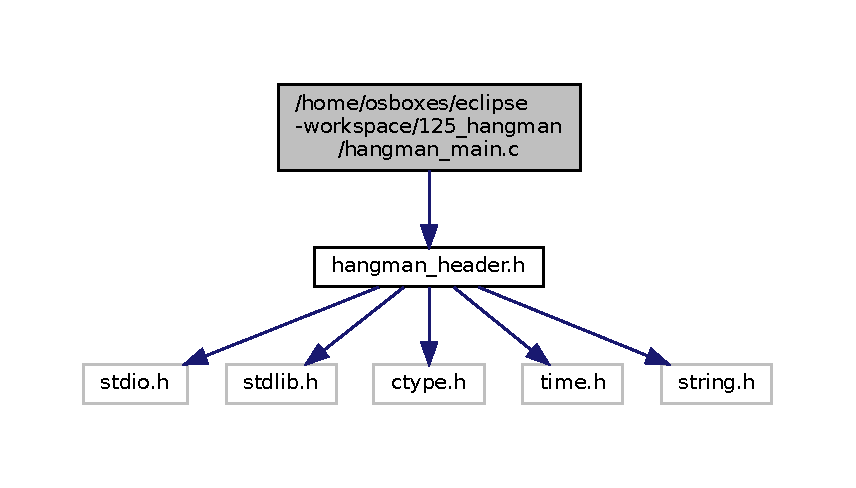
\includegraphics[width=350pt]{hangman__main_8c__incl}
\end{center}
\end{figure}
\subsection*{Functions}
\begin{DoxyCompactItemize}
\item 
int \hyperlink{hangman__main_8c_a0ddf1224851353fc92bfbff6f499fa97}{main} (int argc, char $\ast$argv\mbox{[}$\,$\mbox{]})
\end{DoxyCompactItemize}


\subsection{Function Documentation}
\mbox{\Hypertarget{hangman__main_8c_a0ddf1224851353fc92bfbff6f499fa97}\label{hangman__main_8c_a0ddf1224851353fc92bfbff6f499fa97}} 
\index{hangman\+\_\+main.\+c@{hangman\+\_\+main.\+c}!main@{main}}
\index{main@{main}!hangman\+\_\+main.\+c@{hangman\+\_\+main.\+c}}
\subsubsection{\texorpdfstring{main()}{main()}}
{\footnotesize\ttfamily int main (\begin{DoxyParamCaption}\item[{int}]{argc,  }\item[{char $\ast$}]{argv\mbox{[}$\,$\mbox{]} }\end{DoxyParamCaption})}


%--- End generated contents ---

% Index
\backmatter
\newpage
\phantomsection
\clearemptydoublepage
\addcontentsline{toc}{chapter}{Index}
\printindex

\end{document}
